{$\space$\par}
\vspace{0.5cm}
\justifying
\section*{{\bfseries \LARGE Questão 7 -} {\bfseries \large Aplique uma decomposição de misturas às magnitudes U, B, V, R e I do aglomerado King 5 considerando que cada componente seja uma normal multivariacional.
}}

\vspace{0.3cm}

\begin{enumerate}
    \item Quantas componentes normais multivariacionais são necessárias para explicar a distribuição dessas magnitudes?
        
    \item Quais são as magnitudes médias e a matriz de covariância de cada uma dessas componentes?

    \item Faça dois diagramas cor—magnitude, um ao lado do outro. O primeiro deve ser B−V × V; o segundo deve ser R−I × R. Use o argumento col do comando plot para identificar cada objeto com base na classificação atribuída a ele pela decomposição de misturas.
\end{enumerate}
\vspace{0.8cm}

\textcolor{red}{a) De acordo com o modelo de decomposição de misturas, temos 3 componentes necessárias para explicar a distribuição.}

\begin{lstlisting}
    install.packages('mclust')
    library(mclust)
    model = Mclust(new_df,modelNames = 'VVV')
    summary(model)
    
    ### output ###
    ---------------------------------------------------- 
    Gaussian finite mixture model fitted by EM algorithm 
    ---------------------------------------------------- 
    
    Mclust VVV (ellipsoidal, varying volume, shape, and orientation) model with 3
    components: 
    
     log-likelihood   n df      BIC      ICL
           618.4788 189 62 911.9692 886.6007
    
    Clustering table:
     1  2  3 
    37 85 67 
\end{lstlisting}

\vspace{2em}

\textcolor{red}{b) O vetor das médias pode ser visto no output do código, junto com as matrizes de covariância. Esses valores descrevem completamente as 3 gaussianas multivariacionais encontradas pelo mclust.}

\begin{lstlisting}
    for (i in c(1:3)){
      cat('\nMédia da componente',i,':',model$parameters$mean[,i])
    }
    for (i in 1:3) {
      cat('Matriz componente', i, ':\n')
      print(model$parameters$variance$sigma[,,i])
      cat('\n')
    }
    
    ### output ###
    Média da componente 1 : 19.08092 18.2044 16.9453 16.21884 15.41783
    Média da componente 2 : 18.29859 17.73985 16.61541 15.98515 15.26787
    Média da componente 3 : 20.14439 19.56443 18.22695 17.45339 16.62603

    Matriz componente 1 :
             Umag     Bmag     Vmag     Rmag     Imag
    Umag 3.645411 3.224176 2.959774 2.766449 2.650813
    Bmag 3.224176 3.386730 3.149322 2.955543 2.866553
    Vmag 2.959774 3.149322 2.993255 2.820833 2.780000
    Rmag 2.766449 2.955543 2.820833 2.674180 2.646377
    Imag 2.650813 2.866553 2.780000 2.646377 2.660136
    
    Matriz componente 2 :
              Umag      Bmag      Vmag      Rmag      Imag
    Umag 0.7108262 0.7305238 0.6625979 0.6187826 0.5740213
    Bmag 0.7305238 0.7592262 0.6867012 0.6400591 0.5929057
    Vmag 0.6625979 0.6867012 0.6250097 0.5855402 0.5447514
    Rmag 0.6187826 0.6400591 0.5855402 0.5511798 0.5147319
    Imag 0.5740213 0.5929057 0.5447514 0.5147319 0.4824006
    
    Matriz componente 3 :
              Umag      Bmag      Vmag      Rmag      Imag
    Umag 0.3867627 0.4024006 0.3650820 0.3445183 0.3291485
    Bmag 0.4024006 0.4465300 0.4134285 0.3957304 0.3819135
    Vmag 0.3650820 0.4134285 0.3919677 0.3794756 0.3695648
    Rmag 0.3445183 0.3957304 0.3794756 0.3711844 0.3638454
    Imag 0.3291485 0.3819135 0.3695648 0.3638454 0.3586400
\end{lstlisting}

\vspace{2em}

\begin{figure}[h]
    \centering
    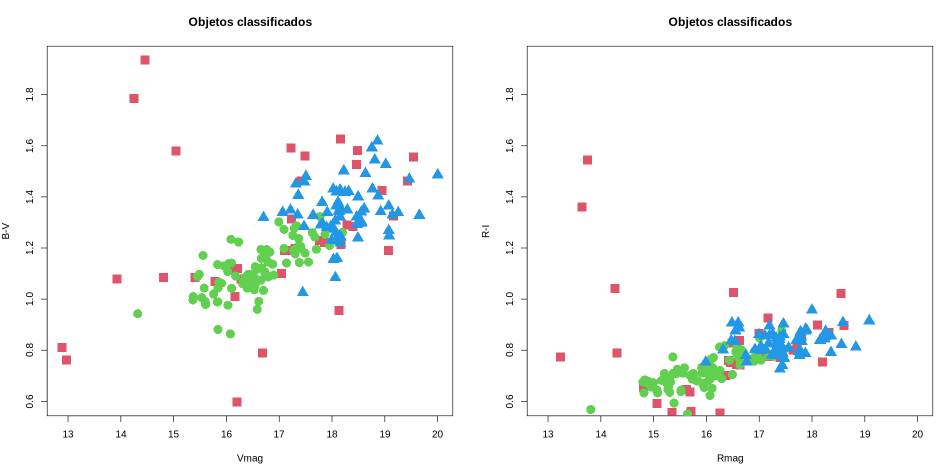
\includegraphics[width=0.8\linewidth]{Figuras/mistura.png}
    \caption{Estrelas do aglomerado aberto King 5 em dois diagramas cor x magnitude. As cores mostram o grupo classificado pela separação de misturas usando o mclust.}
    \label{misturas}
\end{figure}

\textcolor{red}{c) Podemos ver que de fato há 2 populações na imagem \ref{misturas}, onde os objetos do grupo em azul são estrelas mais avermelhadas e com menor brilho aparente, enquanto que o grupo verde são estrelas mais azuladas e maior brilho aparente. Como é um aglomerado e as estrelas devem estar aproximadamente a mesma distância, podemos dizer que esse gráfico se aproxima bastante de um diagrama HR do aglomerado. O terceiro grupo parece ser construídos de outliers, possivelmente objetos fora do aglomerado ou estrelas fora da sequência principal.}

\begin{lstlisting}
    options(repr.plot.width=16,repr.plot.height=8)
    par(mfrow=c(1,2))
    plot(c(), xlim=range(new_df$Vmag), ylim=range(new_df$Bmag - new_df$Vmag),
         xlab="Vmag", ylab="B-V", main="Objetos classificados")
    for (i in c(1:3)){
      sub_df = new_df[model$classification==i,]
      points(sub_df$Vmag,sub_df$Bmag-sub_df$Vmag, col=1+i, pch=14+i,cex=2)
    }
    
    plot(c(), xlim=range(new_df$Vmag), ylim=range(new_df$Bmag - new_df$Vmag),
         xlab="Rmag", ylab="R-I", main="Objetos classificados")
    for (i in c(1:3)){
      sub_df = new_df[model$classification==i,]
      points(sub_df$Rmag,sub_df$Rmag-sub_df$Imag, col=1+i, pch=14+i,cex=2)
    }
\end{lstlisting}


